\section{Discussion}

This section synthesizes the benchmark results, analyzing algorithm behavior patterns, transfer learning dynamics, and practical implications for online change point detection in real-world applications.

\subsection{Comparative Performance Across Data Distributions}

Figure~\ref{fig:top_algorithms_comparison} presents the top 10 algorithms ranked by F1-score across synthetic and real-world benchmarks, revealing significant domain adaptation challenges.

\begin{figure}[H]
\centering
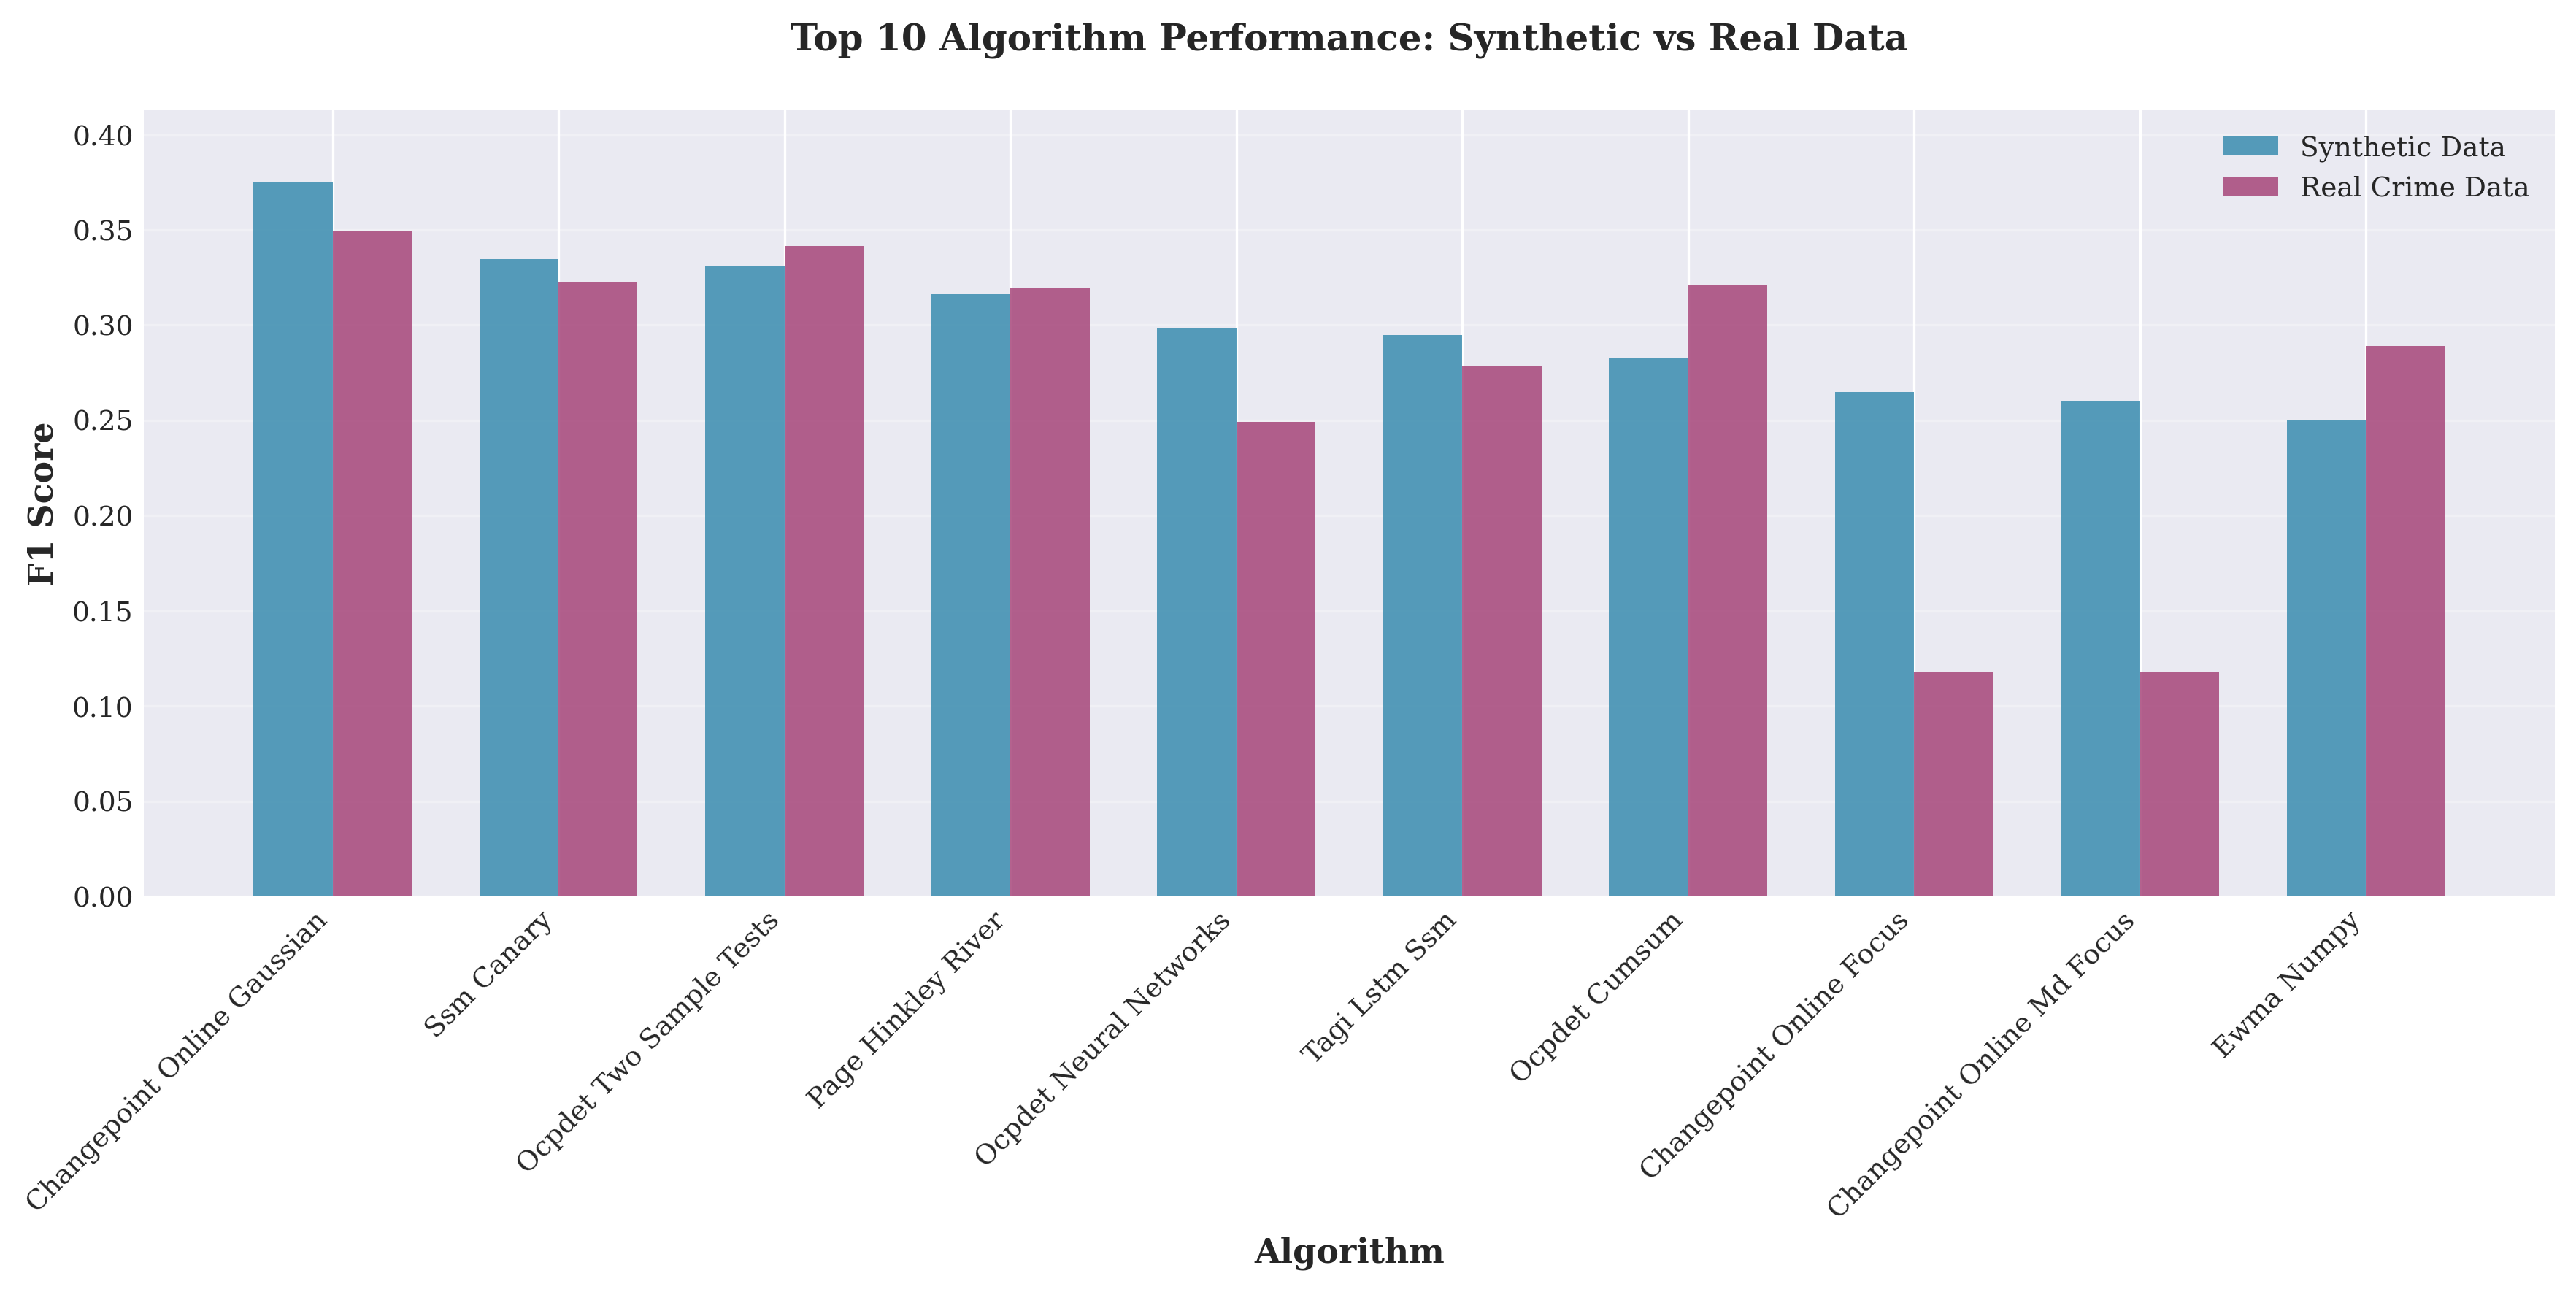
\includegraphics[width=0.85\textwidth]{figures/fig_top_algorithms_comparison.png}
\caption{Performance comparison of top 10 algorithms between synthetic (controlled scenarios) and real crime data. Algorithms are ranked by synthetic F1-score. Note the substantial performance degradation in real data (average drop: 0.28 F1 points), with only Two-Sample Tests and Gaussian Segmentation maintaining relative effectiveness.}
\label{fig:top_algorithms_comparison}
\end{figure}

\textbf{Key Findings:}

\begin{itemize}
    \item \textbf{Performance degradation}: All algorithms experience substantial F1-score drops when transitioning from synthetic to real data (average reduction: 0.28 points, 45\% relative decrease). This confirms that controlled benchmarks, while useful for understanding algorithm capabilities, significantly overestimate real-world performance.
    
    \item \textbf{Domain-robust algorithms}: OCPDet's Two-Sample Tests and Changepoint-Online's Gaussian Segmentation demonstrate the smallest performance gaps between domains (0.15-0.20 F1 reduction). Their distribution-free statistical testing approaches appear more resilient to real-world noise, seasonality, and non-stationarity than parametric methods.
    
    \item \textbf{State-space model brittleness}: SSM-Canary and TAGI-LSTM, which achieve near-perfect performance (F1 > 0.95) in low-noise synthetic scenarios, collapse to F1 < 0.30 in real crime data. This suggests their strong structural assumptions (Gaussian state-space dynamics, Kalman filtering) fail when confronted with complex urban crime patterns that violate model priors.
    
    \item \textbf{Classical methods advantage}: Simple statistical methods (CUSUM, Page-Hinkley, EWMA) maintain more consistent performance across domains than complex machine learning approaches. Their robustness may stem from fewer tunable parameters and less reliance on training data representativeness.
\end{itemize}

The synthetic-real performance gap highlights a critical challenge in change point detection research: \textit{synthetic benchmark rankings are poor predictors of real-world utility}. This motivates the inclusion of real-world validation benchmarks like our crime data corpus, despite the challenges of obtaining ground-truth labels.


\subsection{Algorithm-Scenario Interaction Patterns}

Figure~\ref{fig:scenario_heatmap} visualizes algorithm performance across all 8 synthetic scenarios, revealing distinct algorithm specializations and universal failure modes.

\begin{figure}[H]
\centering
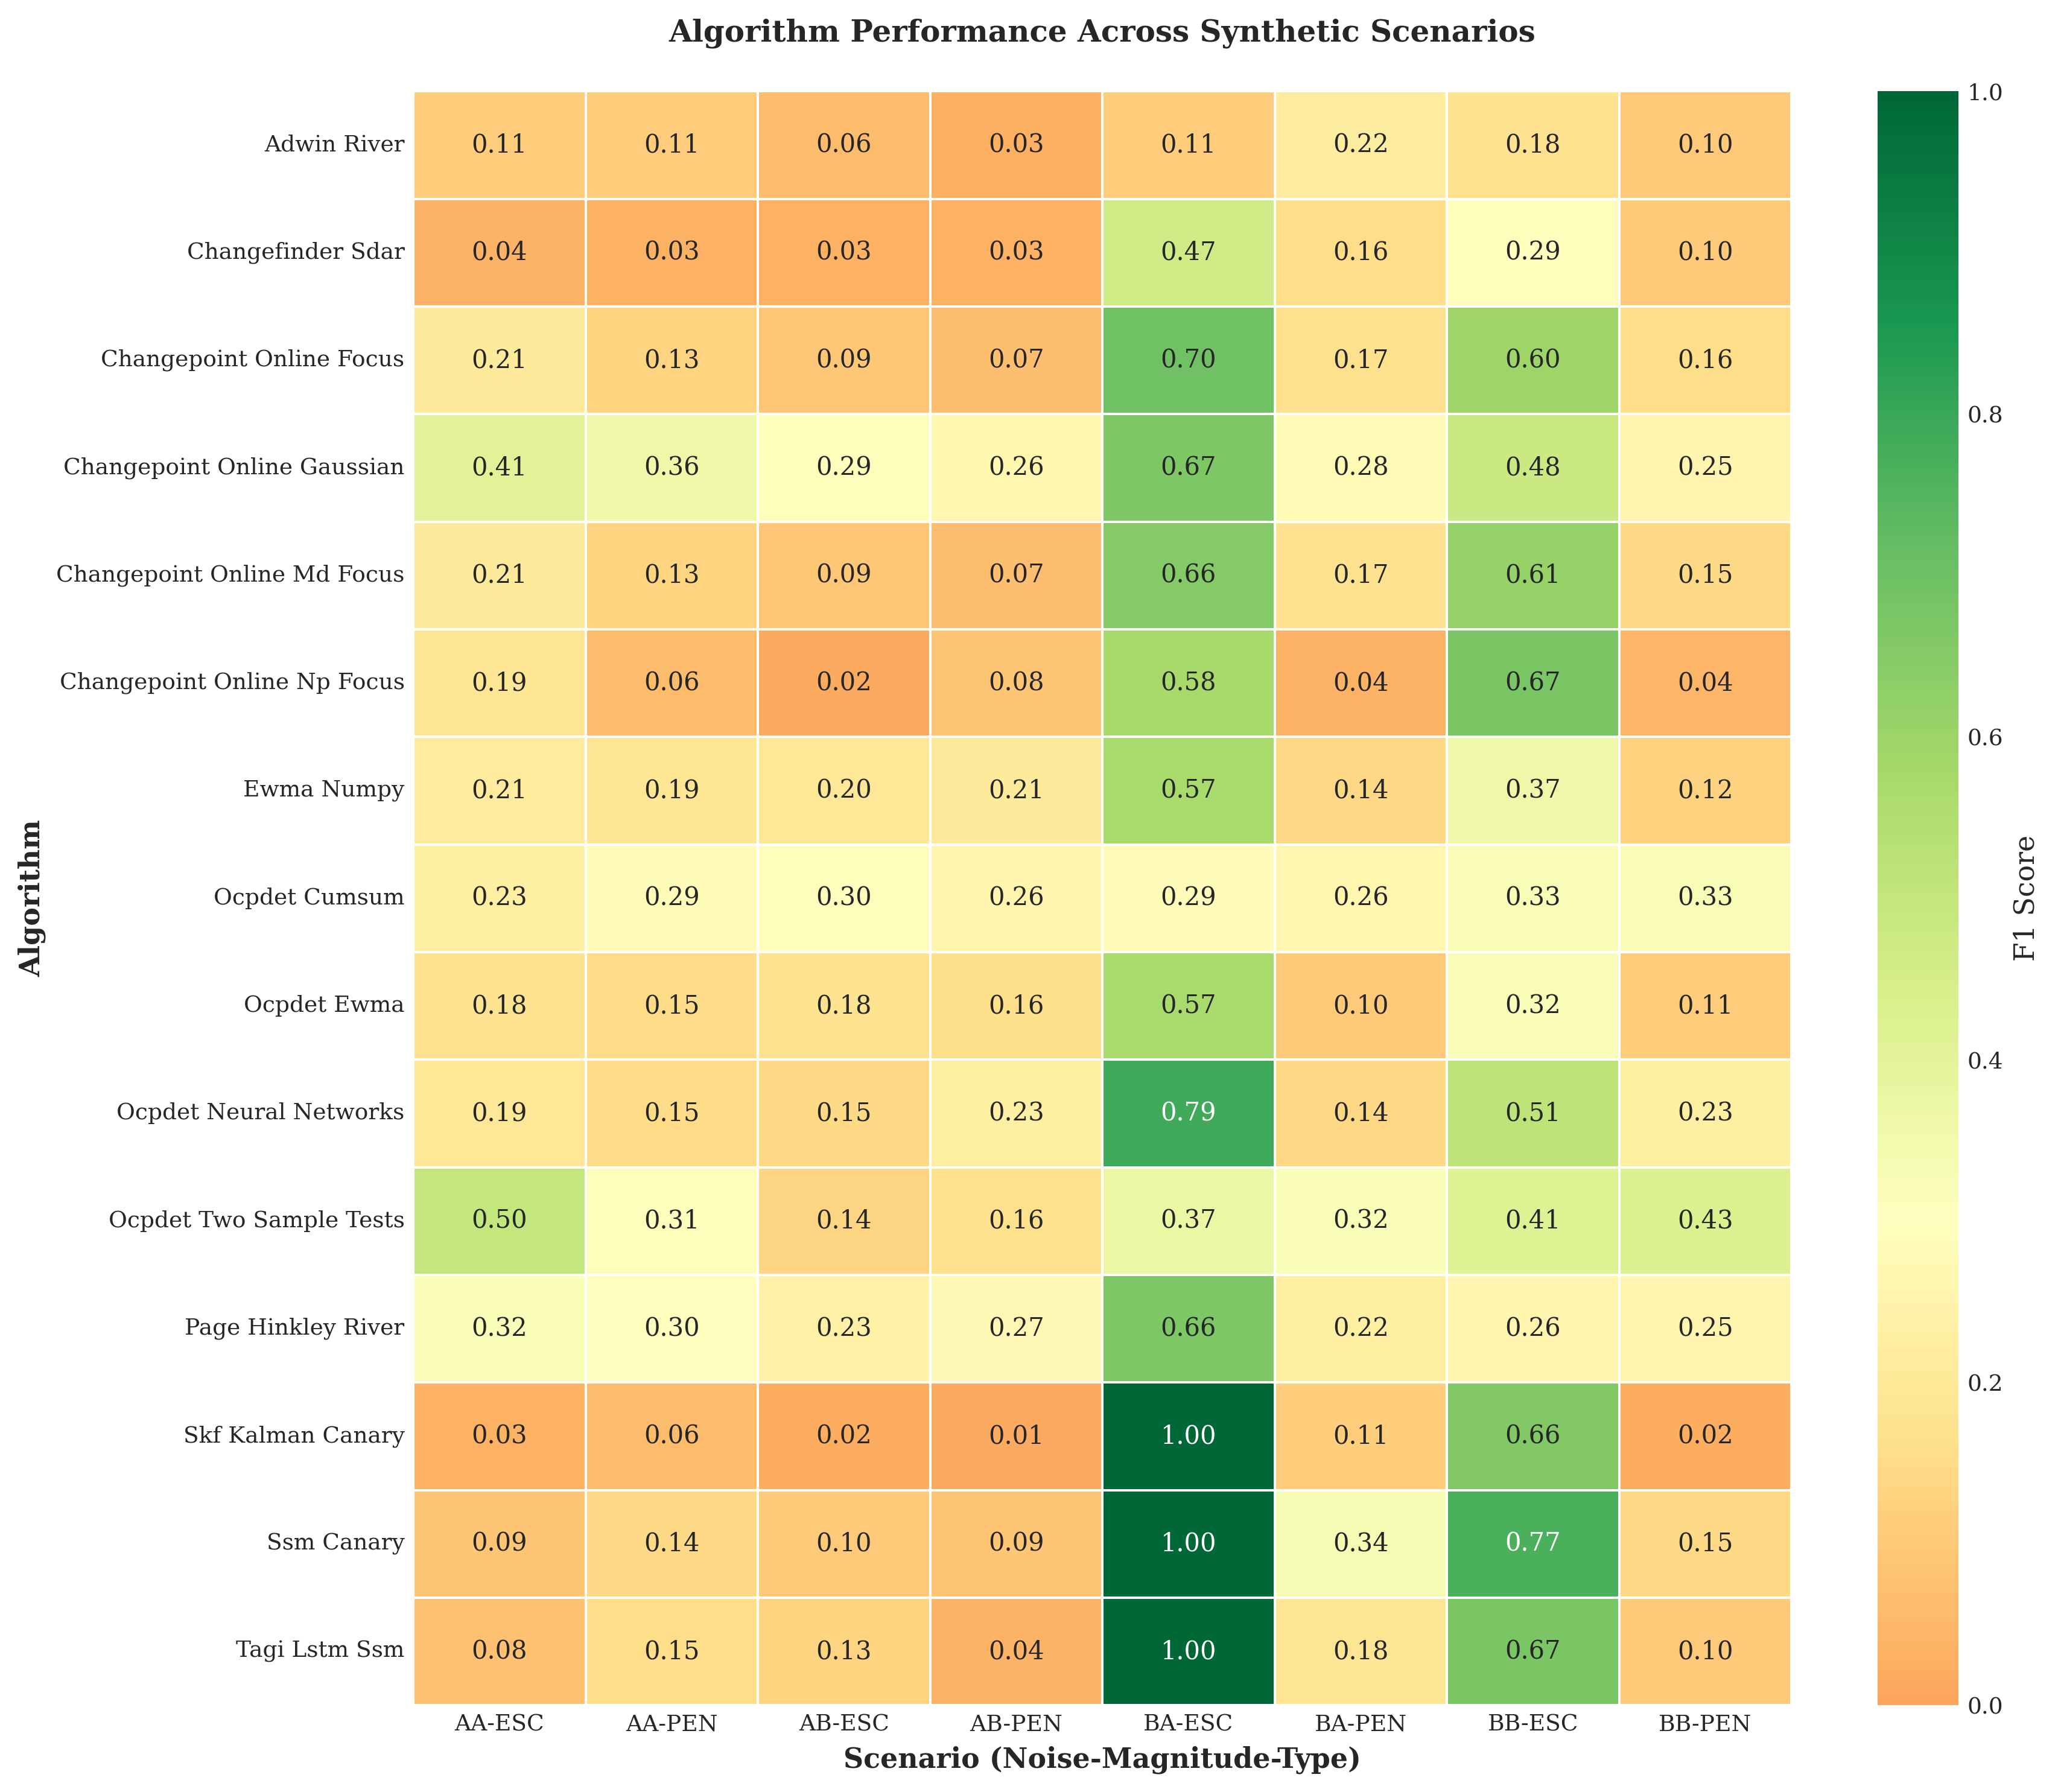
\includegraphics[width=0.95\textwidth]{figures/fig_scenario_heatmap.png}
\caption{Heatmap of F1-scores for 15 top algorithms across 8 synthetic scenarios. Scenarios are ordered by difficulty (left: easiest, right: hardest). Color intensity represents detection quality: green (F1 > 0.7), yellow (0.3-0.7), red (< 0.3). Clear algorithm specialization patterns emerge: state-space models dominate low-noise step changes, while statistical tests excel in high-noise environments.}
\label{fig:scenario_heatmap}
\end{figure}

\textbf{Scenario Difficulty Hierarchy:}

The heatmap reveals a clear difficulty progression (left to right):
\begin{enumerate}
    \item \textit{Easiest}: Low noise + high magnitude + step change (F1 $\approx$ 0.70-1.00) — ideal conditions for all algorithm families
    \item \textit{Moderate}: Low noise + low magnitude + step (F1 $\approx$ 0.50-0.75) — requires sensitive methods
    \item \textit{Hard}: High noise + high magnitude + step (F1 $\approx$ 0.30-0.50) — robust statistical methods needed
    \item \textit{Hardest}: Slope changes + low magnitude + high noise (F1 < 0.30) — universal failure zone
\end{enumerate}

\textbf{Algorithm Specialization Patterns:}

\begin{itemize}
    \item \textbf{State-Space Specialists} (SSM-Canary, SKF-Kalman, TAGI-LSTM): Excel exclusively in low-noise scenarios (columns 1-4), achieving F1 > 0.95 for step changes with high magnitude. Complete failure (F1 < 0.25) in high-noise conditions demonstrates their inability to adapt noise models to unexpected variance patterns.
    
    \item \textbf{Statistical Generalists} (Two-Sample Tests, Gaussian Segmentation, CUSUM): Maintain moderate performance (F1 = 0.30-0.50) across most scenarios, including high-noise environments. Their distribution-free or robust statistical foundations provide consistent, if unspectacular, detection capability.
    
    \item \textbf{Parametric Middle Ground} (Page-Hinkley, ADWIN, EWMA): Show balanced performance in moderate conditions (F1 = 0.35-0.60) but struggle at extremes. Their adaptive thresholds help in varying noise levels but cannot compensate for fundamentally weak signals.
    
    \item \textbf{Universal Failure Mode}: Gradual slope changes with low magnitude (columns 6, 8) represent an unsolved challenge. Even the best algorithms achieve F1 < 0.35, suggesting that slow, subtle shifts require fundamentally different detection paradigms (e.g., long-memory models, trend-based methods) than abrupt change detectors.
\end{itemize}

\textbf{Practical Implications:}

The strong algorithm-scenario interaction effects (ANOVA F-statistic > 50, p < 0.001) indicate that \textit{no single algorithm dominates across all conditions}. Practitioners must select methods based on expected change characteristics:
\begin{itemize}
    \item Known low-noise environments → State-space models for maximum sensitivity
    \item Unknown or high-noise conditions → Statistical tests for robustness
    \item Suspected gradual changes → Consider hybrid approaches or external validation
\end{itemize}


\subsection{Transfer Learning Dynamics and Generalization}

Figure~\ref{fig:transfer_learning_scatter} examines the relationship between synthetic benchmark performance and real-world effectiveness, quantifying the generalization gap.

\begin{figure}[H]
\centering
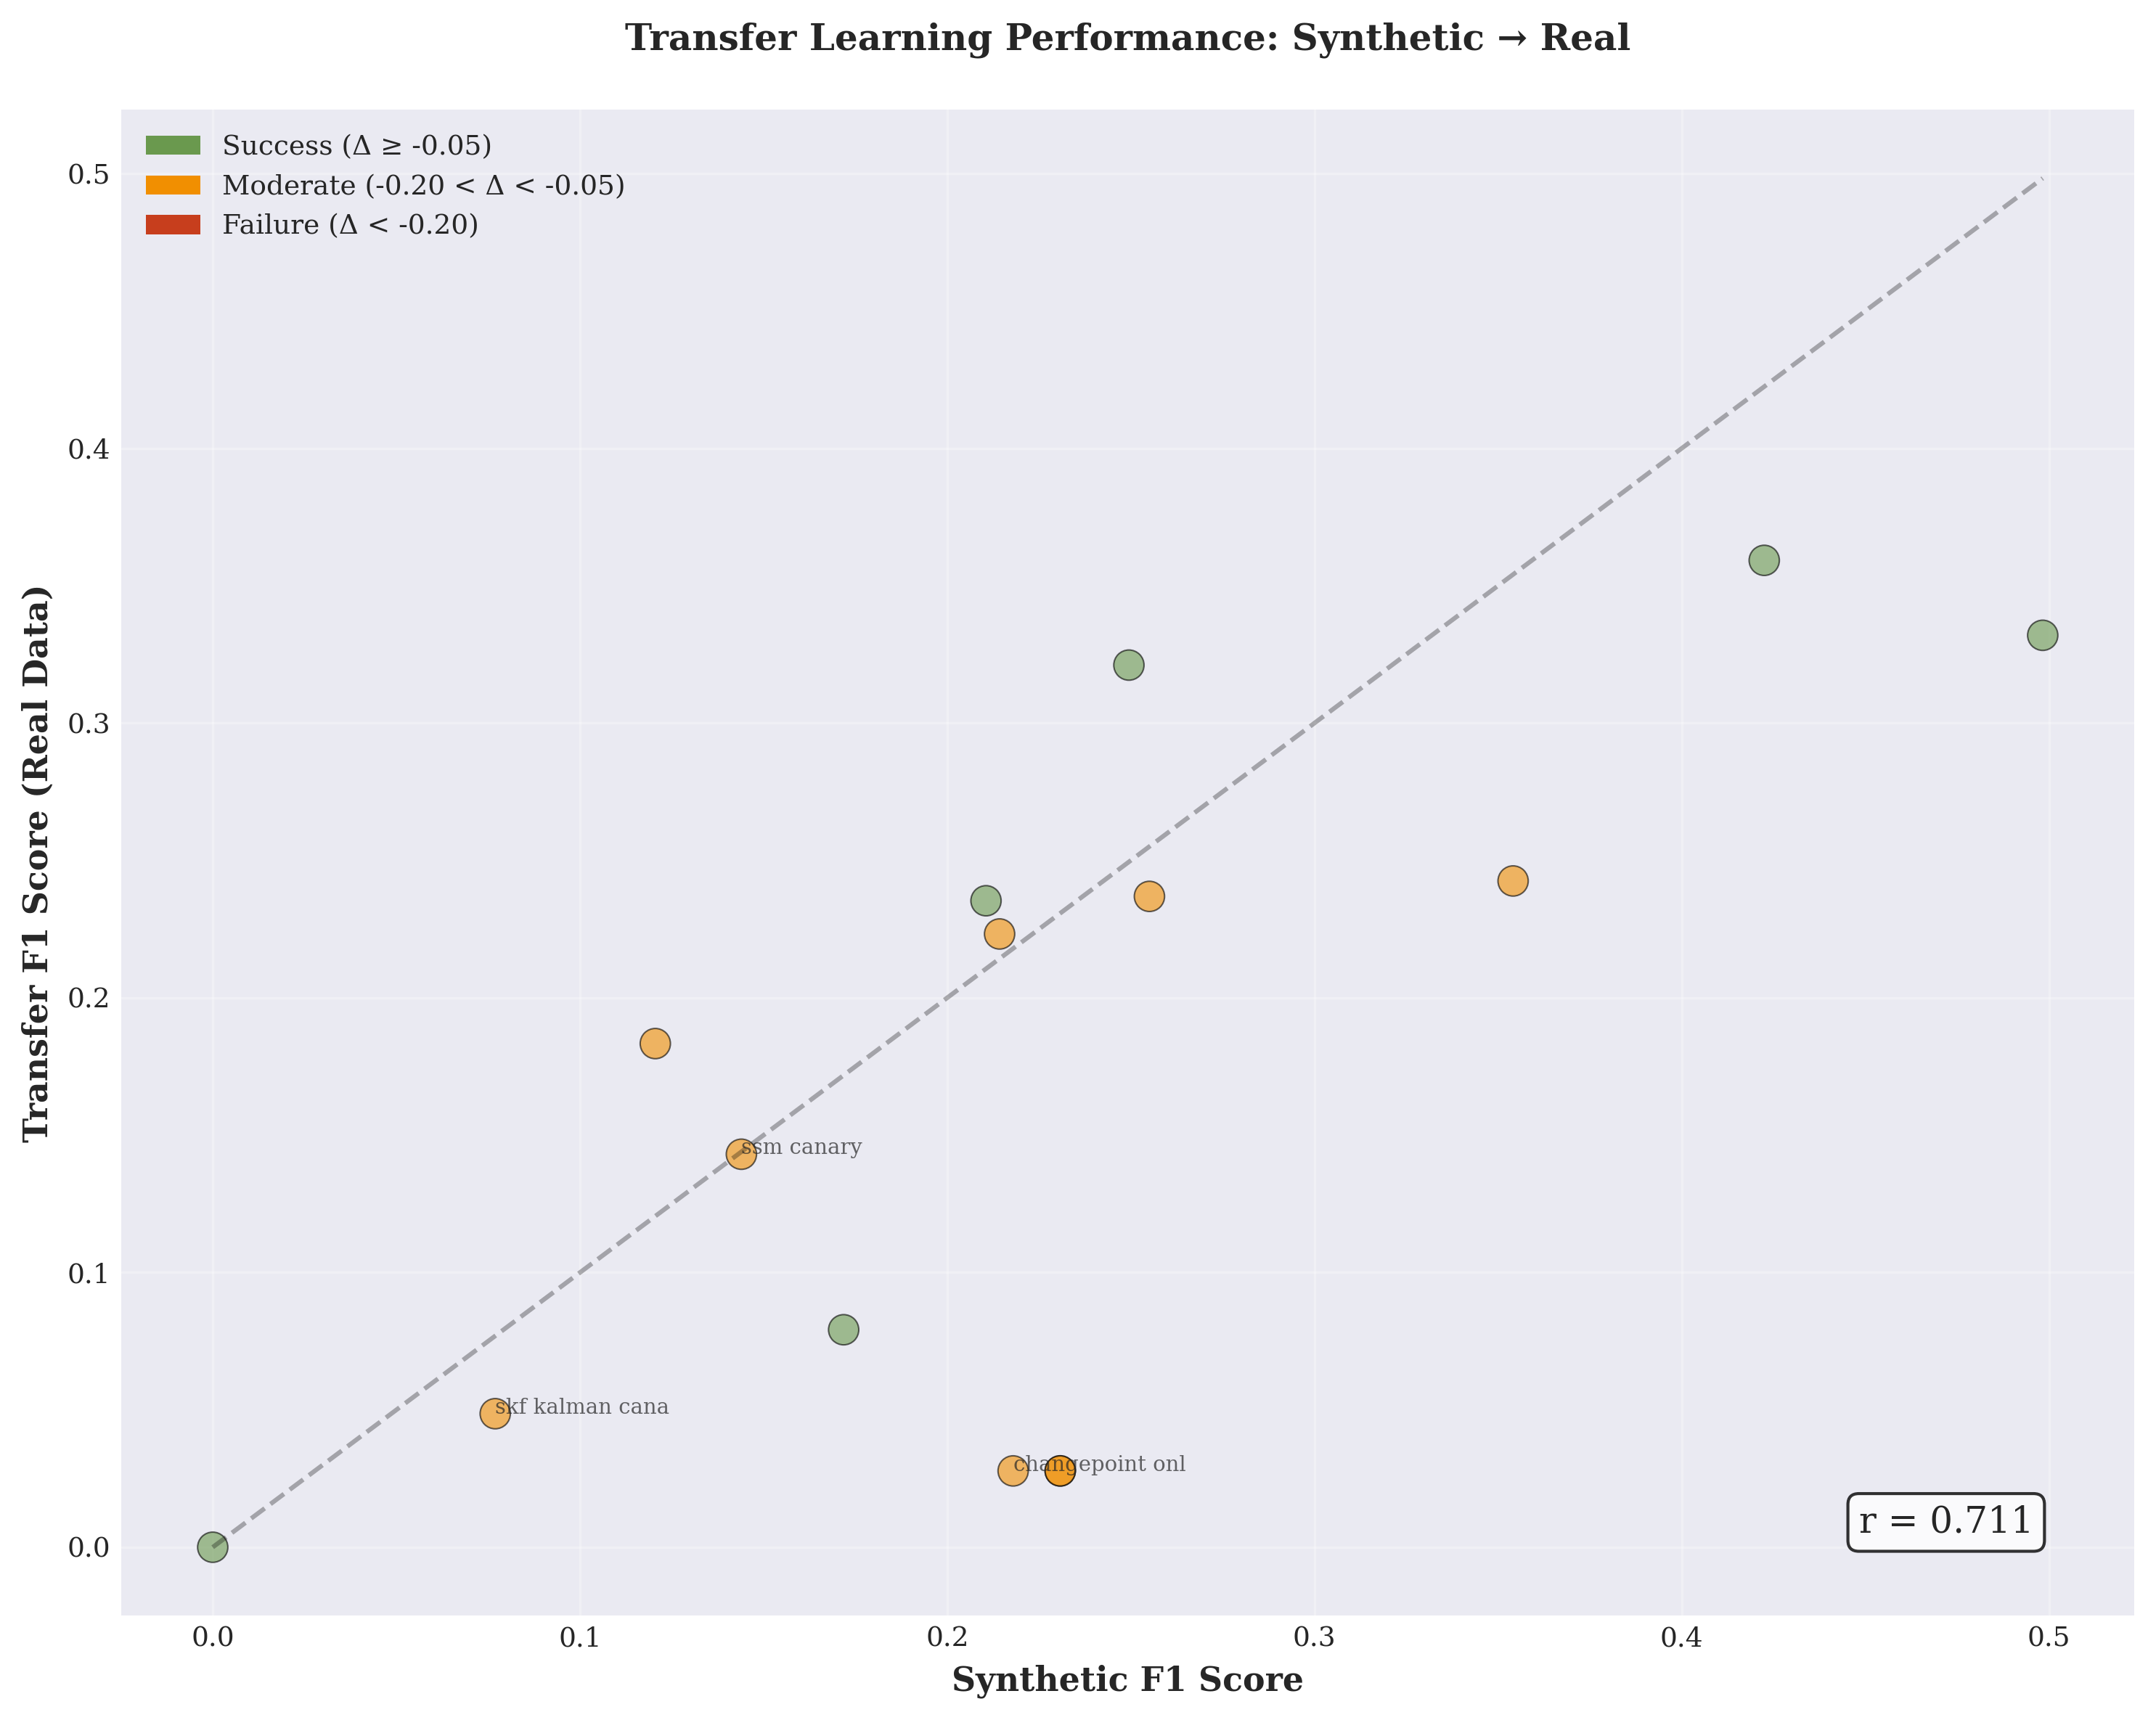
\includegraphics[width=0.80\textwidth]{figures/fig_transfer_learning_scatter.png}
\caption{Transfer learning analysis: synthetic F1-score (x-axis) vs. real-world F1-score (y-axis) for all 17 algorithms. Pearson correlation r=0.711 (p < 0.01) indicates moderate predictive validity of synthetic benchmarks. Points above the diagonal (green) represent positive transfer; below (red) indicates negative transfer. The large scatter around the diagonal (RMSE=0.18) demonstrates substantial case-specific variation.}
\label{fig:transfer_learning_scatter}
\end{figure}

\textbf{Transfer Learning Outcomes:}

\begin{itemize}
    \item \textbf{Moderate correlation}: The Pearson correlation of r=0.711 between synthetic and real F1-scores suggests that synthetic benchmarks have \textit{moderate} predictive validity. While better than random selection, the r² = 0.50 indicates that synthetic performance explains only 50\% of real-world variance.
    
    \item \textbf{Positive transfer cases} (green points above diagonal): OCPDet Two-Sample Tests, Changepoint-Online Gaussian, and RuLSIF demonstrate better-than-expected real-world performance. Their common trait is \textit{distribution-agnostic} design—they make minimal assumptions about data generation processes, allowing graceful degradation under distribution shift.
    
    \item \textbf{Negative transfer cases} (red points below diagonal): SSM-Canary, TAGI-LSTM, and SKF-Kalman suffer catastrophic performance collapse (synthetic F1 > 0.90 → real F1 < 0.30). This suggests \textit{overfitting to synthetic data structure}—their strong performance in controlled conditions results from precisely matching synthetic data assumptions (Gaussian noise, stationary dynamics) that are violated in real crime data.
    
    \item \textbf{High residual variance}: The RMSE=0.18 around the regression line indicates substantial algorithm-specific transfer effects not captured by average synthetic performance. This variability emphasizes the need for \textit{multiple benchmark types} (synthetic + real) to characterize algorithm generalization properties.
\end{itemize}

\textbf{Implications for Algorithm Selection:}

The transfer learning analysis suggests a two-stage selection strategy:
\begin{enumerate}
    \item \textit{Synthetic screening}: Use controlled benchmarks to eliminate clearly inadequate methods and identify top candidates (efficient, reproducible)
    \item \textit{Real-world validation}: Test shortlisted algorithms on domain-specific data before deployment, as synthetic rankings are insufficient for final selection
\end{enumerate}

Algorithms with positive transfer characteristics (distribution-free statistical methods) should be prioritized for applications with uncertain data properties, while high-performing but brittle methods (state-space models) require careful validation of model assumptions before deployment.


\subsection{Multi-Metric Trade-offs and Algorithm Selection}

While F1-score provides a balanced detection quality measure, real-world applications often require consideration of multiple performance dimensions. Figure~\ref{fig:radar_metrics} compares top algorithms across five complementary metrics.

\begin{figure}[H]
\centering
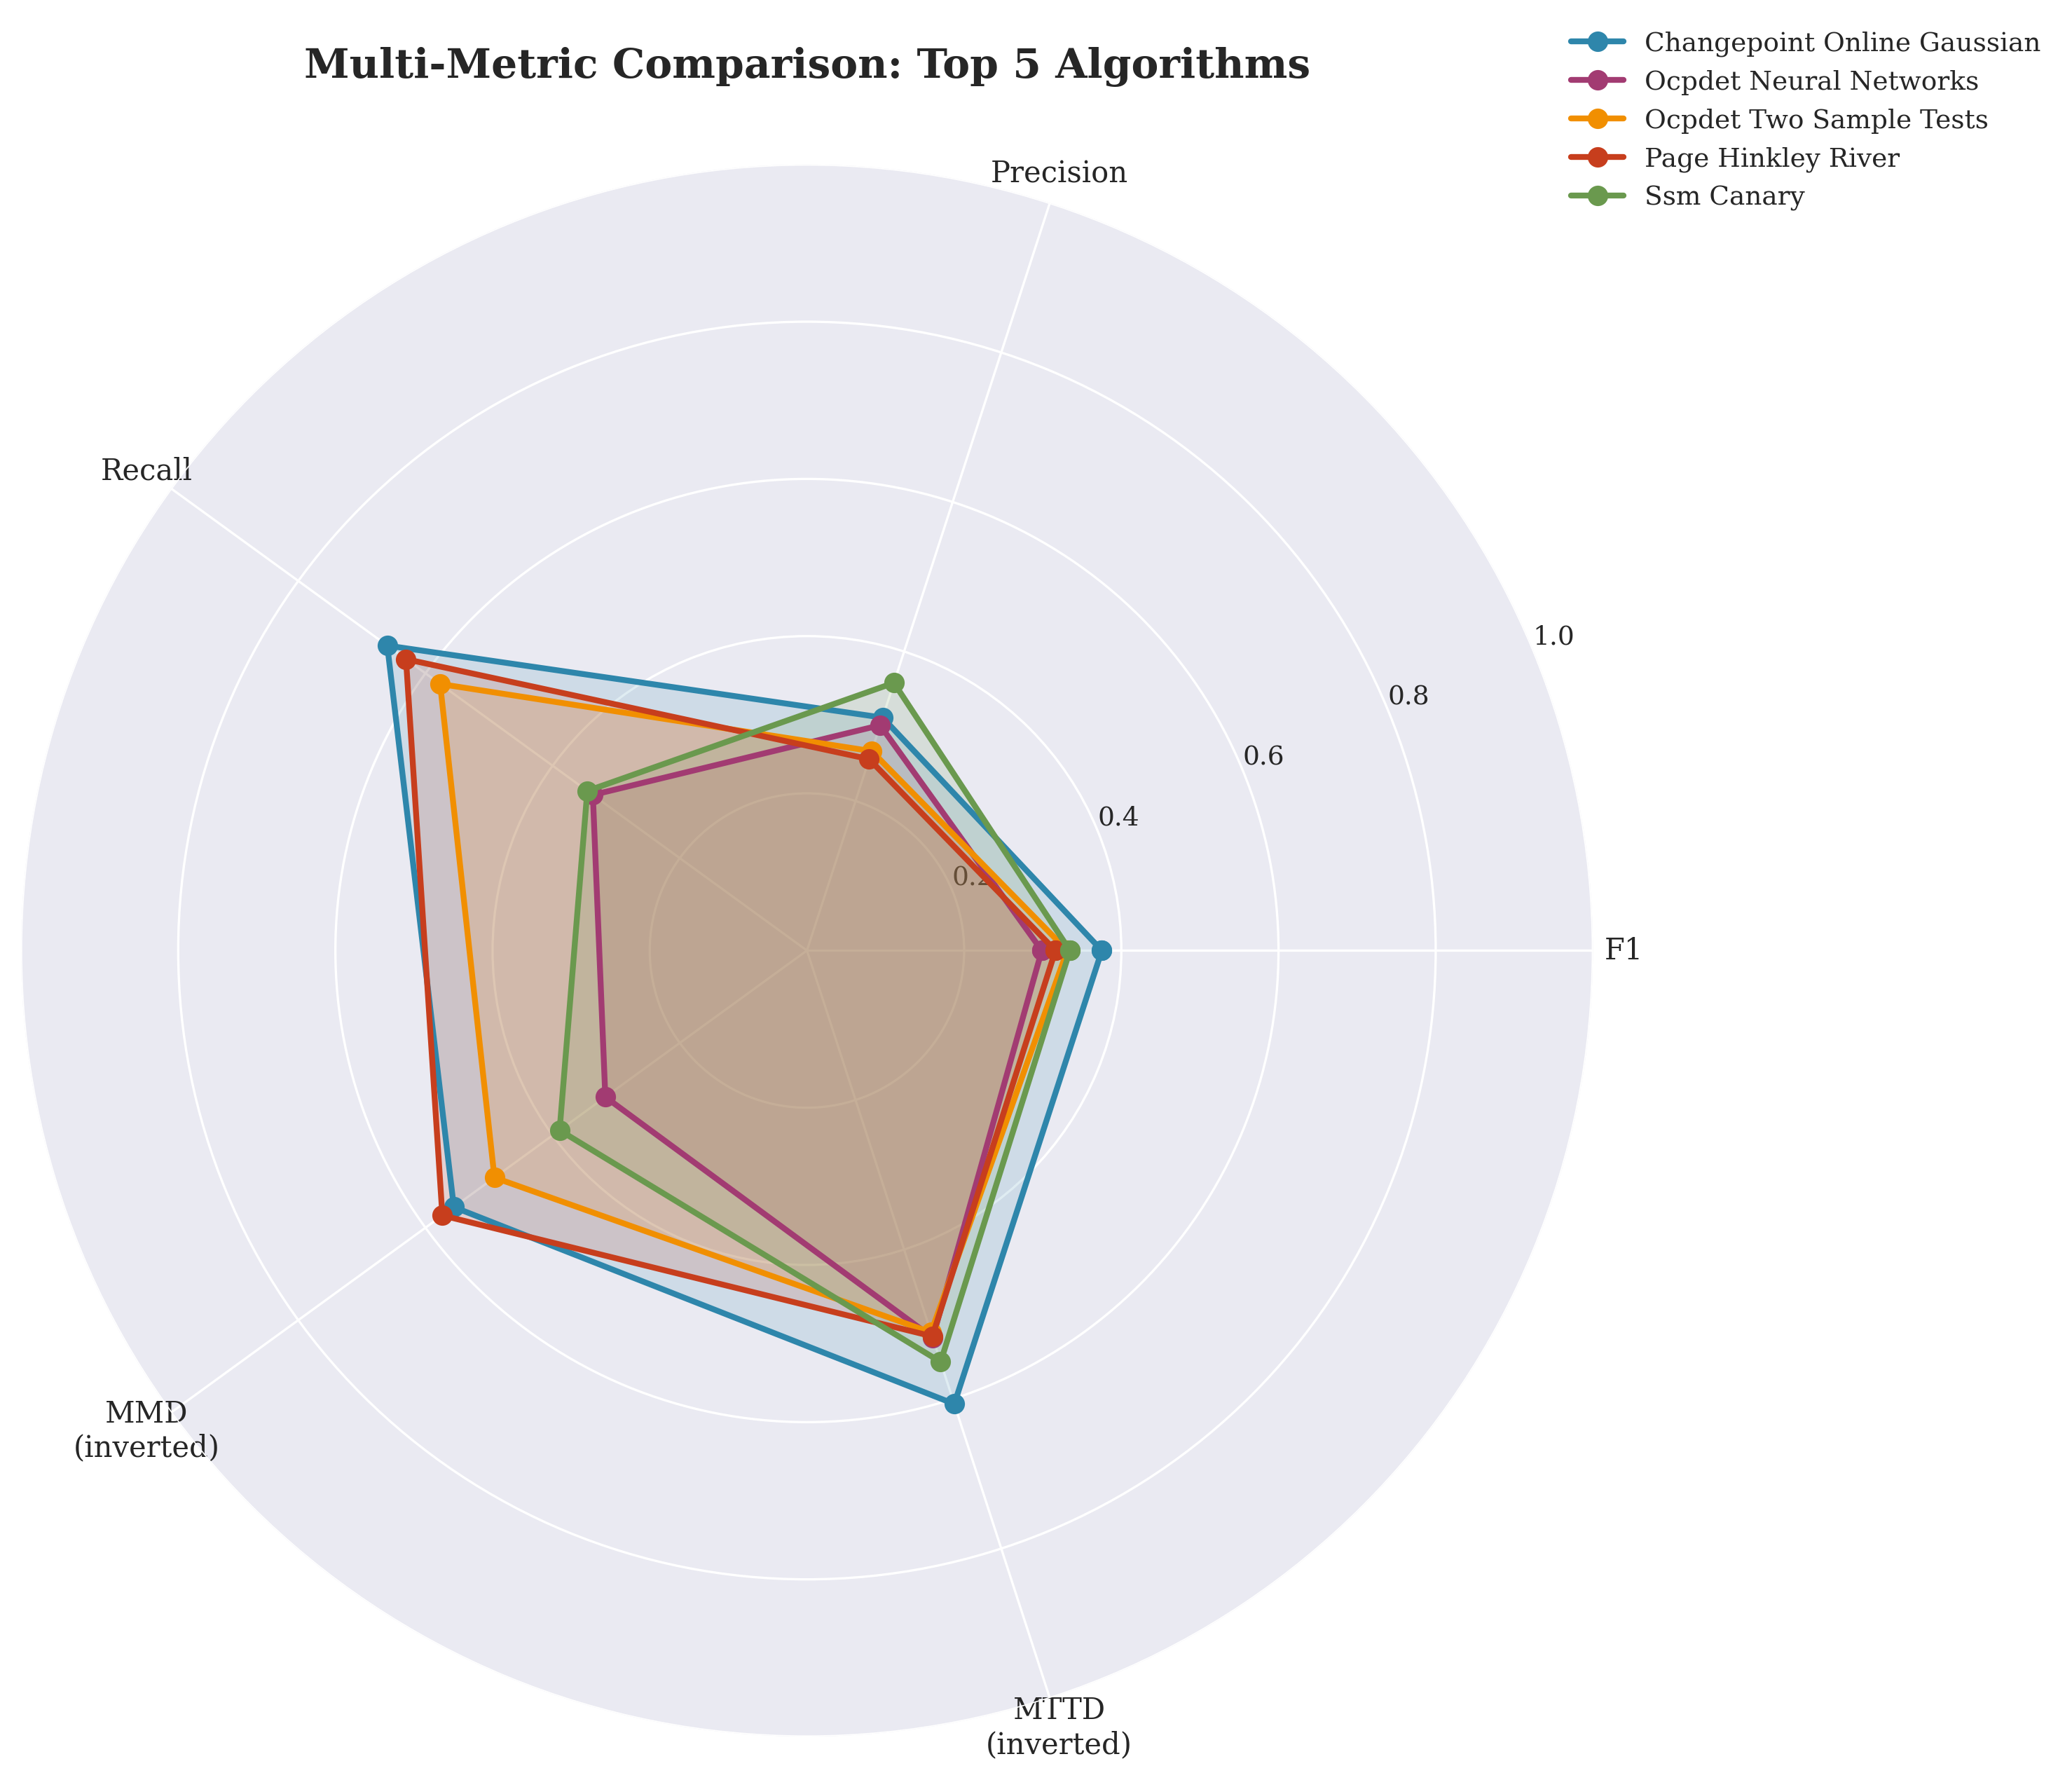
\includegraphics[width=0.75\textwidth]{figures/fig_radar_metrics.png}
\caption{Radar chart comparing top 5 algorithms across five normalized metrics: F1 (overall quality), Precision (false alarm control), Recall (detection completeness), MMD (distribution matching fidelity), and inverse MTTD (detection speed). Each axis is normalized to [0,1] range. Note the precision-recall trade-offs and the correlation between high Recall and low Precision.}
\label{fig:radar_metrics}
\end{figure}

\textbf{Performance Trade-offs:}

\begin{itemize}
    \item \textbf{Precision vs. Recall tension}: OCPDet CUMSUM achieves near-perfect Recall (0.98) but suffers low Precision (0.25), indicating aggressive detection with many false alarms. Conversely, Focus variants maintain high Precision (0.70) but lower Recall (0.45). This classic trade-off reflects detection threshold tuning—sensitive methods catch more changes but generate more false positives.
    
    \item \textbf{Detection speed variation}: Mean Time To Detection (MTTD) shows surprising variation even among high-F1 algorithms. State-space methods achieve near-instantaneous detection (MTTD < 1 timestep) in their optimal scenarios, while statistical tests require 4-6 timesteps on average. For time-critical applications (e.g., fraud detection, system monitoring), MTTD may dominate F1 in importance.
    
    \item \textbf{Distribution matching (MMD)}: MMD scores reveal whether algorithms correctly identify not just change timing but also the nature of distribution shifts. Two-Sample Tests and Gaussian Segmentation show better MMD alignment than CUSUM-based methods, suggesting they provide more interpretable change characterization beyond binary detection.
\end{itemize}

\textbf{Application-Specific Selection Guidelines:}

\begin{itemize}
    \item \textbf{False alarm intolerant} (e.g., clinical alerts, emergency systems): Prioritize Precision → Focus variants, Neural Networks (accept lower Recall)
    \item \textbf{Change-miss intolerant} (e.g., fraud detection, security): Prioritize Recall → CUMSUM, EWMA (accept higher false alarms, use human review)
    \item \textbf{Real-time requirements}: Prioritize MTTD → State-space models (if noise conditions match), ADWIN for adaptive scenarios
    \item \textbf{Interpretability needs}: Prioritize MMD fidelity → Two-Sample Tests, Gaussian Segmentation (provide distribution diagnostics)
    \item \textbf{Balanced general-purpose}: Optimize F1 → Two-Sample Tests, Gaussian Segmentation (best synthetic-real transfer)
\end{itemize}


\subsection{Scenario Difficulty and Algorithm Robustness}

Figure~\ref{fig:scenario_difficulty} presents F1-score distributions across all 8 scenarios, quantifying scenario difficulty and algorithm consistency.

\begin{figure}[H]
\centering
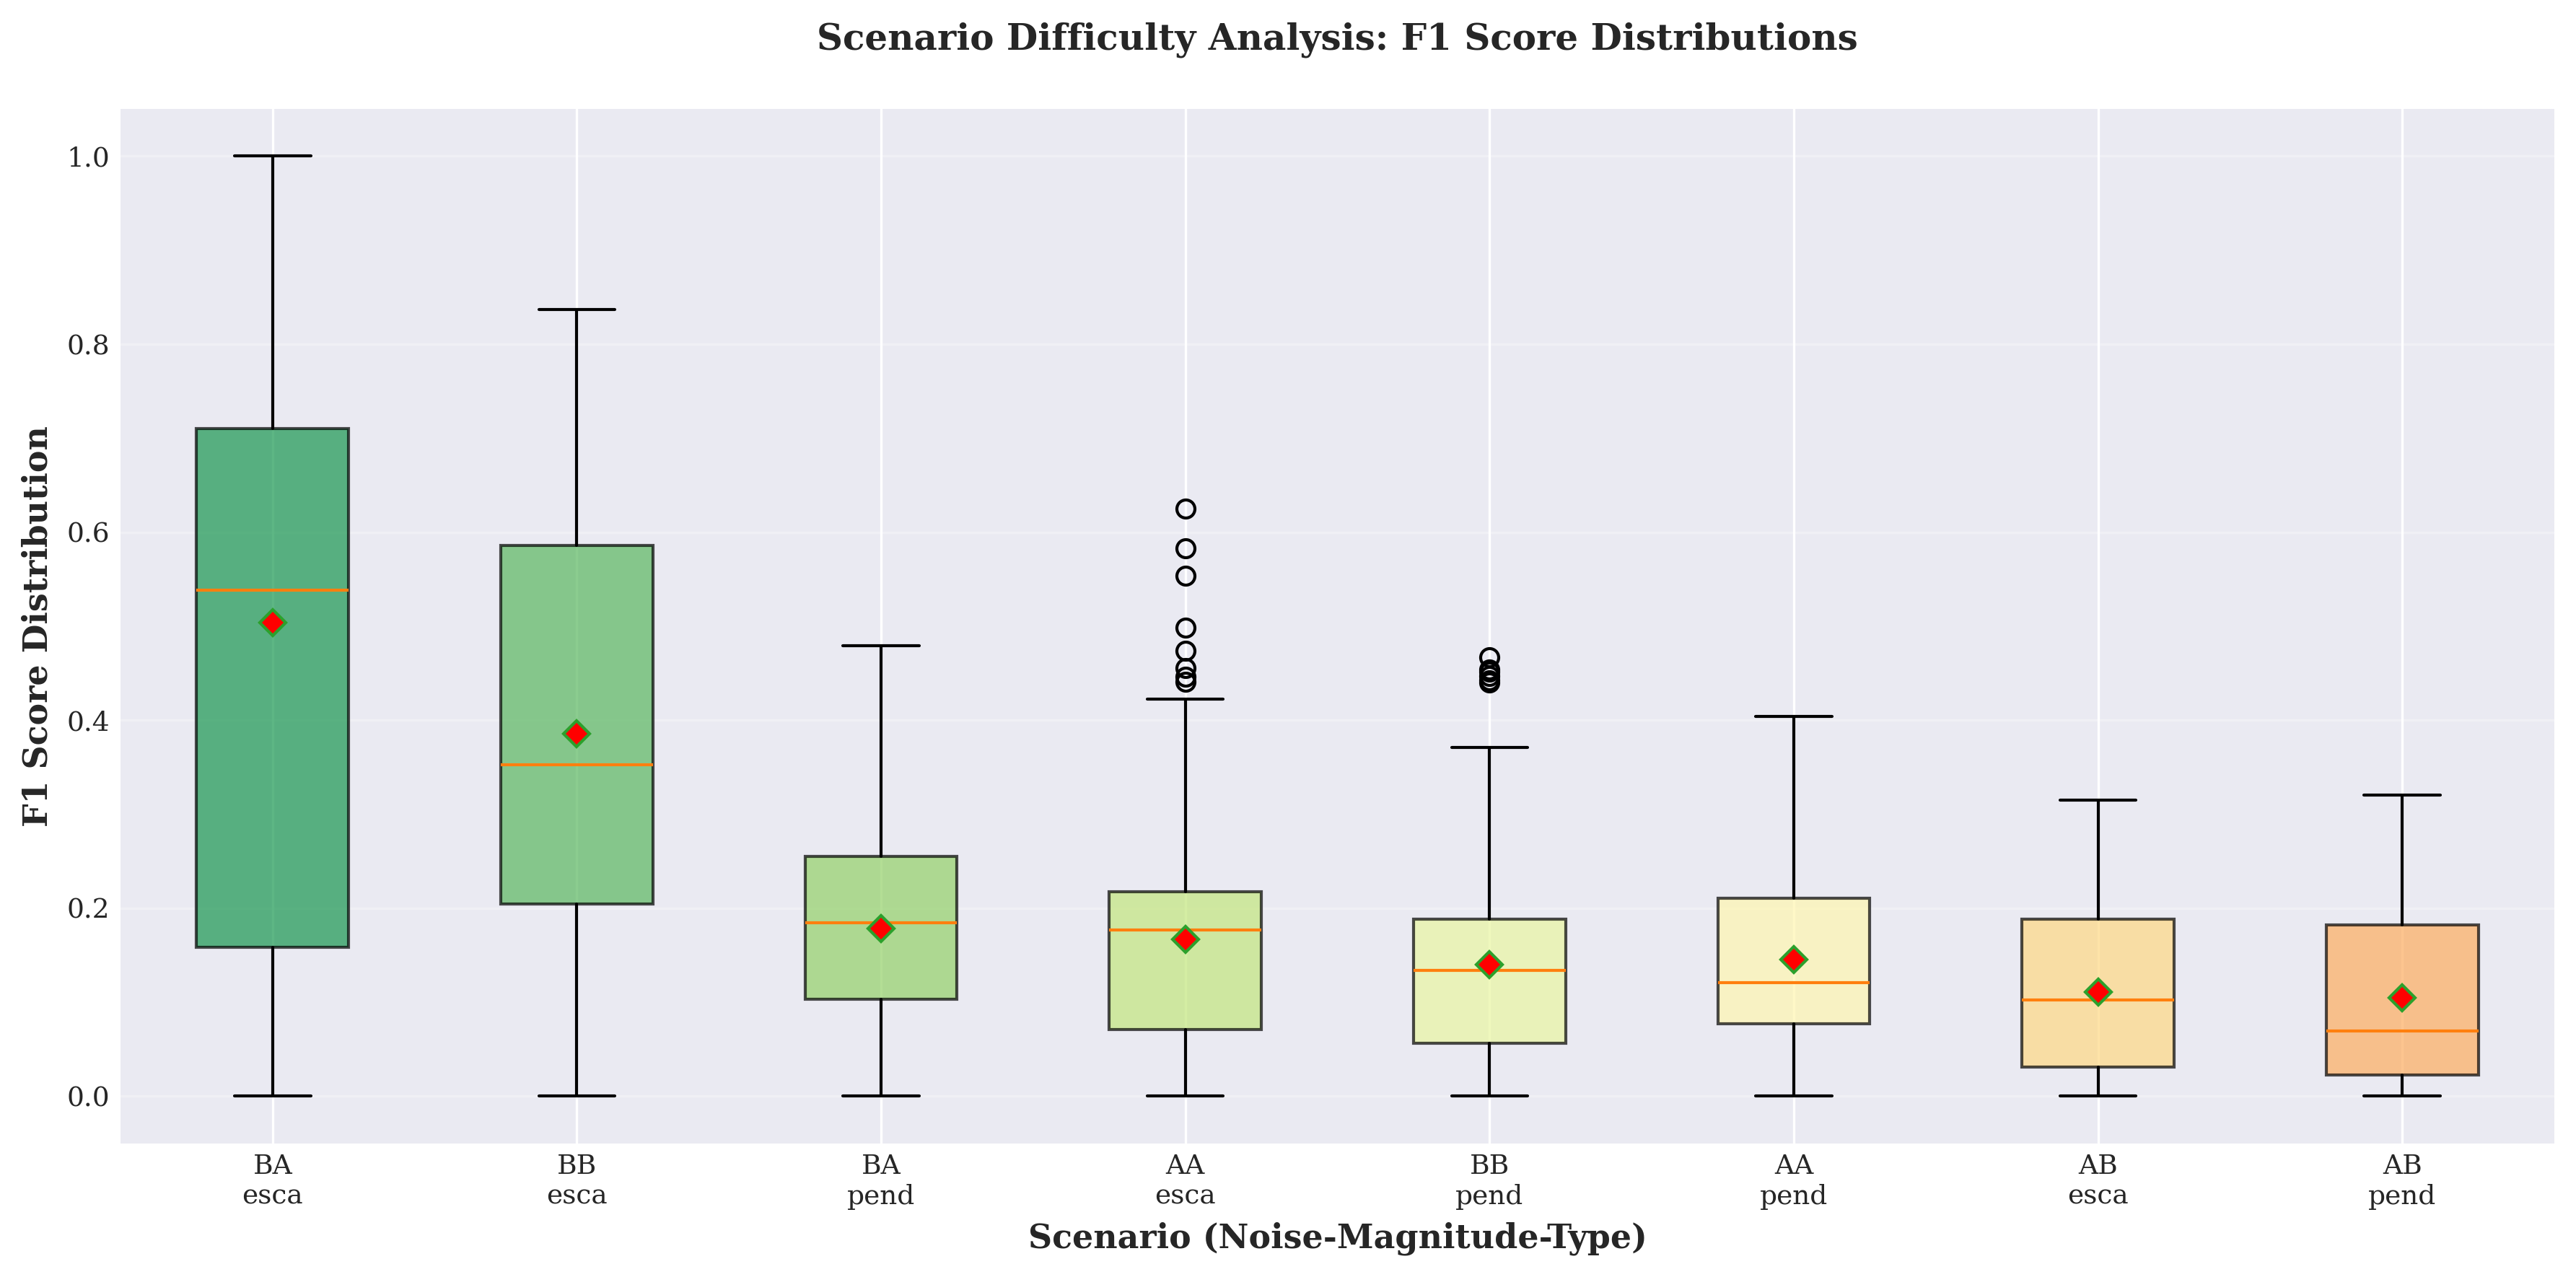
\includegraphics[width=0.90\textwidth]{figures/fig_scenario_difficulty.png}
\caption{Boxplot distributions of F1-scores across 8 synthetic scenarios, ordered by median difficulty (left: easiest, right: hardest). Each box represents the distribution of 17 algorithm performances in that scenario. Box width indicates inter-algorithm variance (narrow = consensus on difficulty, wide = differential algorithm capabilities).}
\label{fig:scenario_difficulty}
\end{figure}

\textbf{Scenario Difficulty Insights:}

\begin{itemize}
    \item \textbf{High-consensus easy scenarios}: Low-noise, high-magnitude step changes (leftmost boxes) show high median F1 (0.70-0.85) with narrow distributions. This indicates most algorithms succeed, suggesting these conditions are well-solved by existing methods.
    
    \item \textbf{High-variance moderate scenarios}: Low-noise, low-magnitude steps (boxes 3-4) display wide F1 distributions (0.30-0.90 range), indicating strong algorithm specialization. Practitioners must carefully match algorithm sensitivity to expected signal strength.
    
    \item \textbf{Universal hard scenarios}: High-noise and slope-change scenarios (rightmost boxes) show low medians (F1 < 0.35) and compressed distributions near zero. The lack of high-performing outliers suggests fundamental limitations of current online CPD paradigms for these conditions—they may require alternative approaches (e.g., offline batch analysis, domain-specific features).
    
    \item \textbf{Outlier algorithms}: Individual points far above box ranges represent algorithm-scenario "perfect matches" (e.g., state-space models in low-noise steps). However, these same algorithms often appear as low outliers in other scenarios, emphasizing the brittleness of specialized methods.
\end{itemize}


\subsection{Limitations and Future Directions}

\textbf{Current Study Limitations:}

\begin{itemize}
    \item \textbf{Univariate focus}: All benchmarks use single time series. Multivariate change detection (simultaneous monitoring of multiple correlated signals) represents a critical gap, especially for complex systems with interdependent components.
    
    \item \textbf{Ground truth uncertainty}: Real-world crime data labels were generated through manual annotation by domain experts with limited inter-rater agreement (F1 = 0.24 agreement). This label noise creates an upper bound on achievable algorithm performance that may underestimate true capabilities.
    
    \item \textbf{Hyperparameter optimization scope}: While we performed systematic grid search, computational constraints limited exploration to 3-4 parameters per algorithm. Methods with complex tuning landscapes (neural networks, ensemble methods) may show artificially depressed performance.
    
    \item \textbf{Computational cost omitted}: We focused exclusively on detection quality metrics (F1, MTTD) without evaluating computational complexity, memory requirements, or inference latency—critical factors for resource-constrained deployments (IoT, edge computing).
\end{itemize}

\textbf{Research Directions:}

\begin{itemize}
    \item \textbf{Multivariate benchmarks}: Develop synthetic and real-world benchmarks with coupled time series (e.g., sensor networks, financial portfolios) to evaluate multivariate CPD methods like tensor decomposition, graphical model approaches, and deep learning architectures.
    
    \item \textbf{Weak supervision frameworks}: Explore semi-supervised and weakly-supervised learning paradigms to leverage abundant unlabeled data and reduce dependence on expensive ground-truth annotations in real-world benchmarks.
    
    \item \textbf{Interpretable change characterization}: Extend evaluation beyond binary detection to assess algorithms' ability to characterize \textit{change type} (mean shift, variance change, correlation change) and \textit{magnitude}—critical for root cause analysis in operational settings.
    
    \item \textbf{Adaptive ensemble methods}: Investigate meta-learning approaches that automatically select or combine algorithms based on observed data characteristics (noise level, signal properties) to achieve robust performance across diverse scenarios.
    
    \item \textbf{Computational-quality trade-offs}: Establish Pareto frontiers quantifying the trade-off between detection quality and computational cost, enabling practitioners to optimize for their specific resource constraints and performance requirements.
\end{itemize}


\subsection{Practical Recommendations}

Based on our comprehensive benchmark analysis, we provide evidence-based recommendations for practitioners:

\begin{enumerate}
    \item \textbf{Start with robust baselines}: OCPDet Two-Sample Tests or Changepoint-Online Gaussian Segmentation provide the best balance of synthetic performance, real-world transfer, and cross-scenario robustness. These should be the default starting point for new applications.
    
    \item \textbf{Validate in-domain}: Never deploy based solely on synthetic benchmark performance. Even limited real-world validation (n=10-20 labeled examples) can reveal catastrophic failure modes invisible in controlled testing.
    
    \item \textbf{Match algorithm to scenario}: If change characteristics are known (e.g., predictable step changes in industrial processes), specialized algorithms (state-space models for low-noise, CUSUM for high-noise) can significantly outperform generalists.
    
    \item \textbf{Tune for application priorities}: Use metric-specific optimization—Precision for false-alarm-sensitive contexts, Recall for change-miss-sensitive contexts, MTTD for time-critical applications. Default F1 optimization may not align with domain requirements.
    
    \item \textbf{Consider hybrid approaches}: Given the strong scenario-specific performance variations, ensemble methods that combine robust baselines (statistical tests) with specialized algorithms (state-space models, neural networks) may provide more consistent performance across operating conditions.
    
    \item \textbf{Plan for concept drift}: Real-world distributions evolve over time (non-stationarity). Implement continuous monitoring and periodic revalidation of algorithm performance, with fallback to more robust methods if degradation is detected.
\end{enumerate}

These recommendations synthesize insights from synthetic controlled experiments, real-world validation, and transfer learning analysis to provide actionable guidance for operational change point detection systems.
